\documentclass{article}

\usepackage{iclr2026_conference,times}
\usepackage{amsmath,amssymb}
\usepackage{booktabs}
\usepackage{graphicx}
\usepackage{microtype}
\usepackage{url}
\usepackage[colorlinks=true,allcolors=blue]{hyperref}

\graphicspath{{figures/}}
\newcommand{\method}{Market Field}
\newcommand{\pressure}{P}
\newcommand{\clip}{\operatorname{clip}}
\newcommand{\EWM}{\operatorname{EWM}}
\newcommand{\EMA}{\operatorname{EMA}}
\newcommand{\med}{\operatorname{median}}
\newcommand{\mean}{\operatorname{mean}}
\newcommand{\R}{\mathbb{R}}

\hypersetup{
  pdftitle={Market Field: An Auditable Multiscale Market-State Instrument for Prospective Option Research},
  pdfsubject={Preliminary systems and methods paper},
  pdfkeywords={financial time series, multiscale representation, non-anticipative computation, relative comparison, options, interpretability}
}
\ifdefined\marketfieldsharecopy
\hypersetup{pdfauthor={Steven J. Meyer}}
\else
\hypersetup{pdfauthor={Anonymous}}
\fi

\title{\method{}: An Auditable Multiscale Market-State\\ Instrument for Prospective Option Research}

\author{
Steven J. Meyer\\
Independent Researcher\\
\url{https://marketdiagnostictool.com}\\
}

\ifdefined\marketfieldfinalcopy
\iclrfinalcopy
\fi

\begin{document}
\maketitle
\ifdefined\marketfieldsharecopy
\lhead{Working paper prepared in ICLR 2026 format}
\fi

\begin{abstract}
Market analysis tools often force a choice between a compact opaque score and an exhaustive but unreadable indicator panel. We ask whether completed market paths can instead be translated into an inspectable answer to four questions: what is moving, how that motion is organized across horizons, how unusual it is relative to the instrument's own fixed history, and how it differs from a chosen reference. We present \method{}, a non-anticipative instrument that maps OHLCV prefixes to a bounded horizon--time field, 15 continuous measurements, a request-local translation dictionary, and an exact-support pairwise comparison. Its design goal is traceable interpretation rather than latent-state discovery or return prediction. Across 32 daily prefix endpoints (6,688 serialized values) and a nine-timeframe supplement (46 endpoints; 24,472 full-precision values), tested channels show zero prefix mismatch, and fixed inputs replay deterministically. Controlled paths exhibit the intended horizon response and trend--chop contrast. The central negative result is equally important: under the same chronology and clustering gate, a cheap five-coordinate baseline forms accepted multi-state codebooks for 8/8 assets with median silhouette 0.448, versus 2/8 and 0.000 for \method{}. Entropy, horizon density, and retained history materially affect the more elaborate coordinates. We therefore conclude that the supported contribution is an auditable measurement and translation protocol, plus infrastructure for a genuinely prospective option study. Current field snapshots have zero direct scanner authority; a separately governed historical-learning canary is capped at 10\%. Predictive, economic, and human-comprehension value remain questions to test, not properties implied by the mathematics.
\end{abstract}

\section{The Goal: Make a Market-State Claim Inspectable}

A price can rise while short-horizon pressure fades, long-horizon structure remains organized, realized variation expands, and performance versus a benchmark stalls. A single score erases those distinctions. A conventional indicator panel preserves them only by asking the reader to reconcile many windows, scales, and units unaided. Options add another separation problem: a contract can appear cheap under the current optionality heuristic while the underlying path is poorly aligned with the thesis.

The goal of \method{} is to produce a compact market-state conclusion that can be traced back through its visible evidence, measured definitions, support, and completed inputs. The target reader questions are:
\begin{enumerate}
    \item What direction is the path taking, and is that direction strengthening or fading?
    \item Is the move coherent across horizons or concentrated and disordered?
    \item Is the current measurement ordinary or stretched relative to a fixed proper-fit history?
    \item How does the same measurement differ from a chosen reference on exact shared alignment keys?
\end{enumerate}
The intended output is a description that guides inspection, not a scalar recommendation.

\begin{figure}[t]
    \centering
    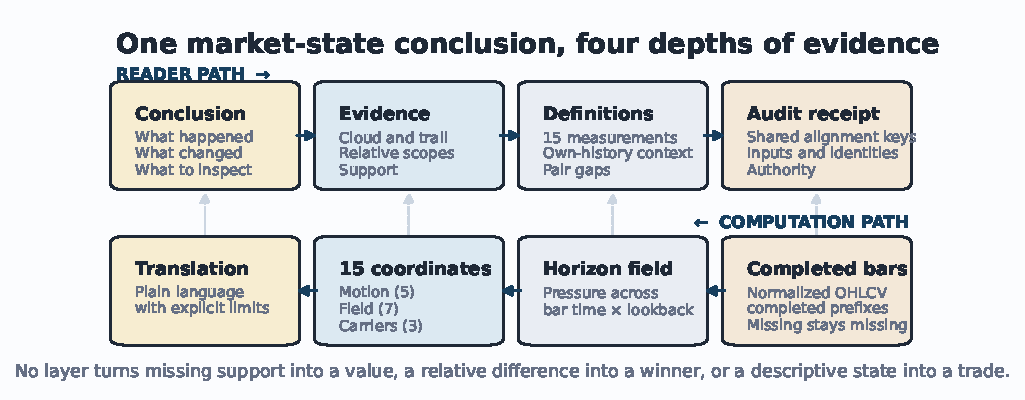
\includegraphics[width=\linewidth]{research_contract.pdf}
    \caption{The information hierarchy used by the paper and research interface. A reader begins with a conclusion and can drill into evidence, definitions, and a receipt. Computation moves in the opposite direction from completed observations. Missing support remains unavailable throughout the stack.}
    \label{fig:research-contract}
\end{figure}

We ask whether this instrument can satisfy four requirements before its decision value is known: \emph{non-anticipation} (live measurements use only the completed prefix), \emph{reconstructibility} (definitions and identities can be replayed), \emph{semantic traceability} (each model-generated state phrase has a declared evidence mapping), and \emph{bounded authority} (descriptive context cannot silently become a trade rule). Formula v1 fixes the numerical construction; semantic revision 1.3 adds support, identity, and authority evidence without changing those values. Exact version names are collected in Appendix~\ref{app:versions}.

The contribution is a complete instrument rather than a claim that mathematical complexity is intrinsically useful:
\begin{enumerate}
    \item a bounded multihorizon path representation and 15-coordinate measurement vocabulary;
    \item a conclusion--evidence--definition--receipt translation contract, including own-history and pairwise reference context;
    \item a falsification-oriented audit containing prefix tests, controlled paths, a matched cheap baseline, and parameter/resolution sensitivity; and
    \item prospective option-research instrumentation that preserves eligibility and execution boundaries while future evidence accumulates.
\end{enumerate}

\section{What Each Layer Means}
\label{sec:reader-contract}

Table~\ref{tab:questions} makes the interpretation contract explicit. Its first four rows are the descriptive questions in Section~1; the final row is a prospective downstream research question, not a fifth core output. Higher does not generally mean better: disorder, realized-variation state, participation, and liquidity stress are measured quantities rather than utilities. The interface therefore shows a model-generated state conclusion first, then lets the reader inspect the exact coordinate, its history, its support, and the transformation that produced it.

\begin{table}[t]
\centering
\small
\setlength{\tabcolsep}{3.5pt}
\begin{tabular}{p{0.20\linewidth}p{0.32\linewidth}p{0.39\linewidth}}
\toprule
Reader question & Evidence & Meaning boundary \\
\midrule
What is moving? & Pressure and bounded time derivatives & Measured directional path state; not expected return. \\
How is it organized? & Structure, information, geometry, propagation & Cross-horizon agreement and change; not market physics or a detected cycle. \\
How unusual is it? & Fixed-fit coordinates and held-out calibration-distance rank & Relative to one retained history; not a universal regime or formal p-value. \\
How does it differ? & Native coordinate gap, own-history-relative gap, relative price & Different questions on timeframe-specific exact shared keys; none supplies a ``winner.'' \\
\midrule
Prospective: does it fit an option thesis? & Optionality evidence beside side-aligned path context & A condition to study; not eligibility, sizing, or execution. \\
\bottomrule
\end{tabular}
\caption{The translation contract. Each conclusion names its evidence and the strongest interpretation that evidence supports.}
\label{tab:questions}
\end{table}

\paragraph{Relationship to prior work.}
SwamiCharts arrange a common indicator across lookbacks \citep{ehlersway2012introducing,ehlersway2012strategies}; wavelets, scattering transforms, and multifractal models provide principled multiscale alternatives \citep{mallat2012scattering,andenmallat2014deep,bacry2001multifractal}. \method{} retains the visual scan across scale but uses a causal EMA/true-range/path-efficiency construction suited to interactive inspection. Markov-switching, structural-break, and online change-point models estimate latent or discontinuous states \citep{hamilton1989new,baiperron1998structural,adamsmackay2007bocpd}; the present Forms are instead request-local compression labels. Scope plots borrow the intuition of phase and recurrence views \citep{takens1981detecting,eckmann1987recurrence,marwan2007recurrence}, while permutation entropy is the directly adopted nonlinear statistic \citep{bandtpompe2002permutation}. Implied-versus-realized volatility and variance-risk-premium research motivates the optionality question \citep{carrwu2009variance,bollerslev2009variance,goyalsaretto2009options}; the open contribution is whether independently measured path context improves prospective decisions, not a new definition of volatility mispricing.

\section{Constructing the Instrument}
\label{sec:method}

\subsection{A bounded field over time and horizon}

Let $O_t,H_t,L_t,C_t,V_t$ be a sorted, deduplicated OHLCV prefix, $M_t=(H_t+L_t)/2$, and $h_1<\cdots<h_J$ an ordered horizon grid. A gap-aware true range normalizes the displacement between fast and slow exponential averages, and path efficiency discounts movement that travels far but ends near its start:
\begin{align}
z_{j,t} &=
\frac{\EMA_{\max(2,\lfloor h_j/2\rfloor)}(M)_t-\EMA_{h_j}(M)_t}
     {\operatorname{Mean}_{h_j}(TR)_t}, &
d_{j,t}&=\frac{z_{j,t}}{1+|z_{j,t}|}, \label{eq:direction}\\
e_{j,t} &=
\clip_{[0,1]}
\frac{|M_t-M_{t-h_j}|}{\sum_{i=t-h_j+1}^{t}|M_i-M_{i-1}|}. \label{eq:efficiency}
\end{align}
Equation~\ref{eq:efficiency} follows Kaufman's efficiency-ratio construction \citep{kaufman1995smarter}. Causal time smoothing and adjacent-row blends produce bounded pressure $\pressure_{j,t}$: its sign describes direction and its magnitude combines displacement with path organization. Horizon density is part of formula v1 because row adjacency changes when the grid changes. Appendix~\ref{app:calculus} specifies every coefficient, missing-value convention, edge rule, and the prefix-measurability argument.

Causal bounded differences form pressure change, acceleration, jerk, and snap. Numerical derivatives over $u_j=\log h_j$ describe scale gradient, curvature, and their temporal change. Five motion coordinates, seven field coordinates, and three OHLCV carriers then form $\mathbf{x}_t\in\R^{15}$. The field family separates:
\begin{itemize}
    \item \textbf{motion}: direction and how quickly that direction is changing;
    \item \textbf{organization}: agreement, disorder, geometry, and propagation across horizons; and
    \item \textbf{carriers}: realized variation, volume participation, and an Amihud-like price-impact ratio \citep{amihud2002illiquidity}.
\end{itemize}
The kinematic terms are mnemonic labels for normalized finite differences. The scope views are measured trajectories, not inferred attractors or cycles.

\subsection{Translation without replacing the measurements}

The 15 coordinates remain the authoritative values. A deterministic dictionary is fitted only on a proper-fit segment, with a later segment reserved for state-conditional distance calibration and a final segment for evaluation. Family-balanced robust scaling and farthest-point-initialized $k$-means \citep{macqueen1967methods,gonzalez1985clustering} consider at most five Forms; support and mean-silhouette gates \citep{rousseeuw1987silhouettes} fall back to one Form when separation is weak. Forms are compact names for calibration-relative profiles, not persistent market regimes.

For evaluation distance $d_t$ assigned to Form $k$, the empirical upper-tail rank is
\begin{equation}
\tau_t=\frac{1+\#\{d_i^{\mathrm{cal},k}\ge d_t\}}{n_k+1}.
\label{eq:tail}
\end{equation}
The display calls $\tau_t<0.05$ with $n_k\ge20$ the \emph{upper state-conditional calibration-distance tail}. This is a same-state distance rank, not coordinatewise range, density support, or a forecast. Every coordinate separately reports whether a finite value was computed, whether its declared dependencies are fully supported, and whether an internal neutral placeholder was used. A phrase is withheld when its required evidence is unavailable.

\subsection{Own-history and chosen-reference context answer different questions}

Relative Field Pair v1 independently builds target $A$ and reference $B$ under the same recipe, then aligns timeframe-specific exact shared keys on bilateral support. The direct coordinate difference
\begin{equation}
\Delta^{\mathrm{native}}_{j,t}=X^A_{j,t}-X^B_{j,t}
\end{equation}
compares the implemented coordinate scale. The own-history-relative difference
\begin{equation}
\Delta^{\mathrm{context}}_{j,t}
=\frac{X^A_{j,t}-m^A_j}{s^A_j}
-\frac{X^B_{j,t}-m^B_j}{s^B_j}
\end{equation}
asks which instrument is more elevated relative to its separate fixed proper-fit history. Normalized relative price is displayed separately. Missing or provisional cells are never coerced to zero, and request-local Forms are never matched across instruments. The ordered receipt freezes shared keys, support, references, and zero authority. Appendix~\ref{app:relative-pair} and the standalone technical addendum give the exact alignment, beta-context, reset, and hash contracts.

The current interface presents one of four relationship scopes at a time: directional phase, higher motion, structure--information, or propagation--carriers. Chronological opacity follows source time rather than screen position; unsupported runs stay broken; start and current markers require true supported endpoints. A shared scale supports comparison, while an inspection scale may zoom the selected trail. These are translation choices over unchanged coordinate values.

\begin{figure}[t]
    \centering
    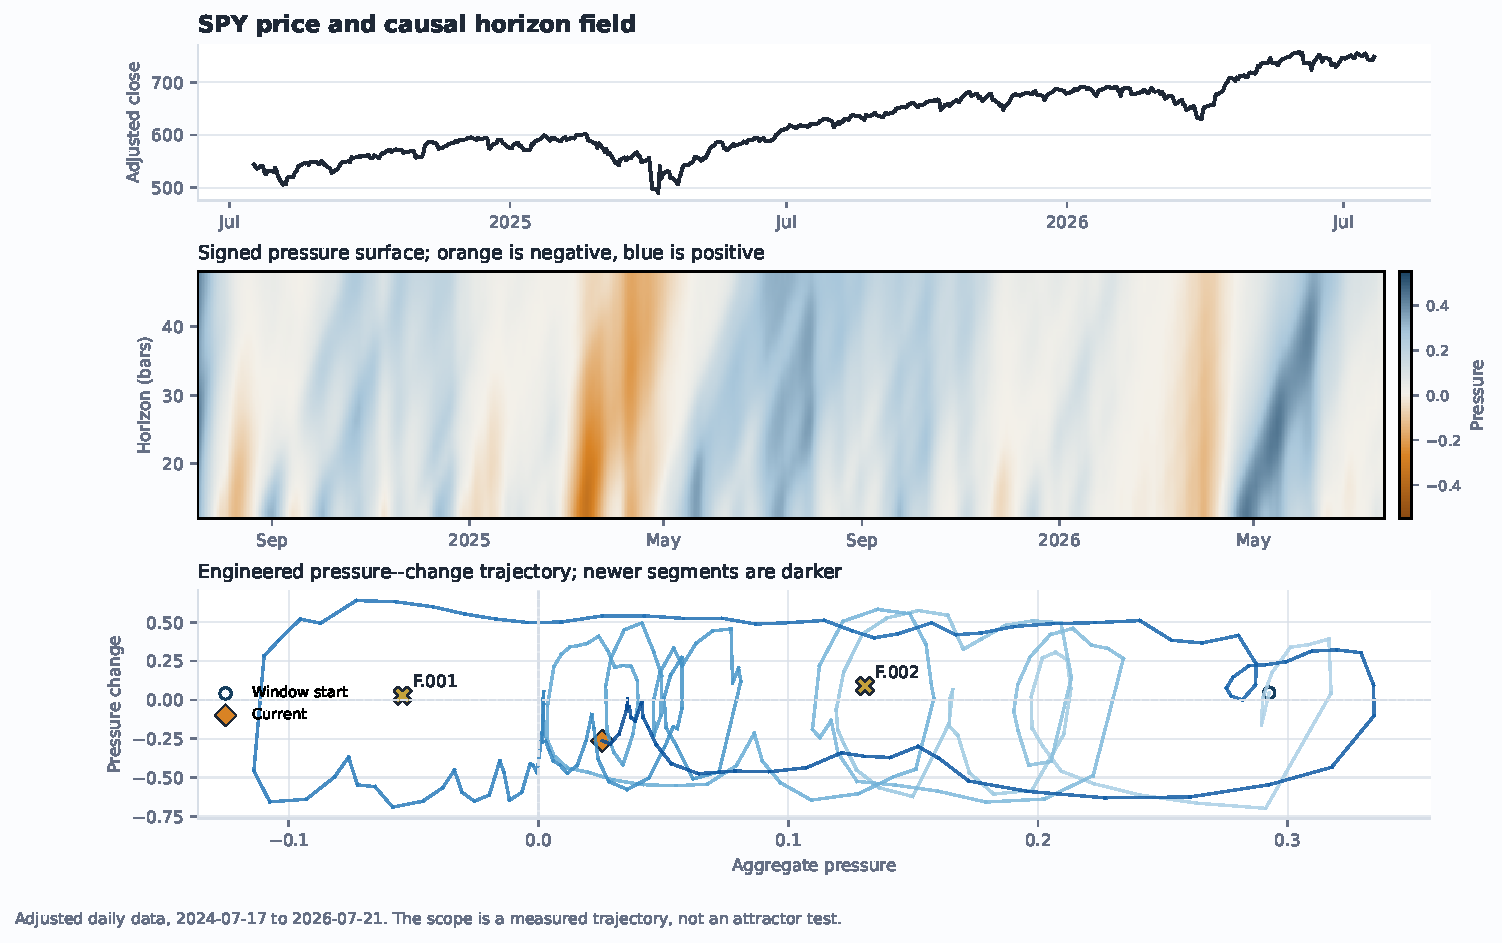
\includegraphics[width=\linewidth]{spy_field_phase.pdf}
    \caption{SPY over the final 500 daily bars. Price alone shows the path level; the horizon field exposes intervals of positive and negative pressure across scale; the pressure--change projection shows how the measured state moved. Request-local centroids label this history only.}
    \label{fig:field}
\end{figure}

\section{Evaluation: Does the Instrument Behave as Claimed?}
\label{sec:evaluation}

The evaluation is organized around the goal rather than around every equation:
\begin{description}
    \item[Integrity] Do tested live measurements depend only on the available prefix, and do fixed inputs replay?
    \item[Construct meaning] Do controlled paths produce the directional and cross-horizon responses the interface describes?
    \item[Incremental structure] Does the 15-coordinate representation form cleaner or more stable unsupervised states than a cheap five-coordinate baseline?
    \item[Robustness] How strongly do entropy window, horizon density, and retained history change the result?
\end{description}
Integrity addresses non-anticipation and reconstructibility; controlled paths and declared phrase-to-evidence mappings address semantic traceability; Pair and option authority receipts and metamorphic checks address bounded authority. Incremental structure and robustness are additional falsification tests rather than implied parts of those four contract requirements.
Economic and human-comprehension value are deliberately separated from these representation tests.

The primary audit uses adjusted daily Yahoo Finance OHLCV from 2018-01-01 through 2026-07-21 for SPY, QQQ, IWM, TLT, GLD, USO, VNQ, and BTC-USD. A locally retained supplement covers 15 datasets and all nine supported SPY timeframes. Normalized snapshots and derived artifacts are hashed; provider restrictions prevent redistribution of the original raw files. Exact execution lineage and rerun limits appear in the reproducibility package.

Prefix tests rebuild 11 channels across 19 horizons at four cut points per asset and compare the same endpoints with the later suffix present. Fixed-input replay compares canonical dictionary hashes. Controlled constructions include an 800-bar reversal and a matched trend-versus-alternating-chop path. The baseline uses five causal 24-bar features---EMA displacement, EMA slope, signed path efficiency, realized variation, and volume---under the same warm-up, fit/calibration/evaluation split, robust scaling, deterministic clustering, support gate, and silhouette threshold.

\subsection{The measured computation is prefix-consistent and responds as designed}

\begin{figure}[t]
    \centering
    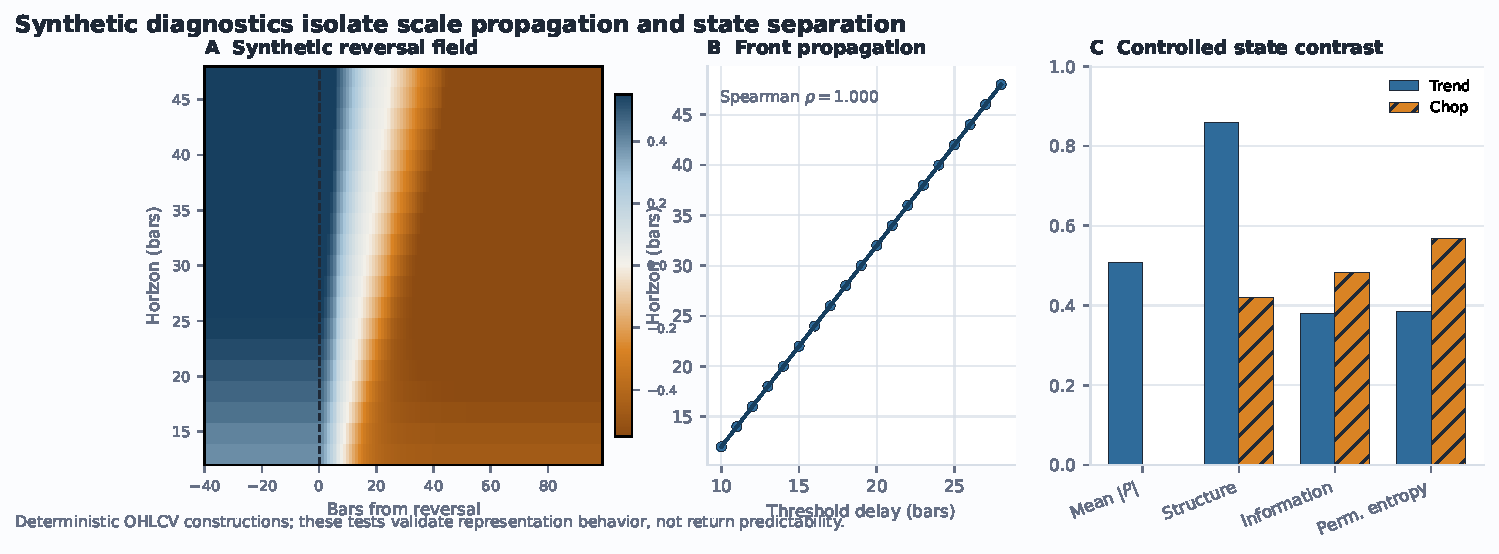
\includegraphics[width=\linewidth]{synthetic_diagnostics.pdf}
    \caption{Controlled construction evidence. The reversal travels from short to long horizons, and organized trend differs from alternating chop in the intended measurements. These panels validate the translation's constructed meaning, not a return forecast.}
    \label{fig:synthetic}
\end{figure}

\begin{table}[t]
    \centering
    \small
    \setlength{\tabcolsep}{3pt}
    \begin{tabular}{p{0.30\linewidth}p{0.23\linewidth}p{0.39\linewidth}}
\toprule
Diagnostic & Result & Interpretation \\
\midrule
Prefix invariance & 6,688 comparisons, 0 mismatches & No future-bar dependence detected at $10^{-4}$ API precision. \\
Deterministic dictionary & 8/8 exact reruns & Fixed inputs yield byte-identical versioned lexicons. \\
Synthetic propagation & $\rho=1.000$ & Longer horizons cross the reversal threshold later by construction. \\
Distance-tail diagnostic & 1.5--10.6\% by asset & State-conditional empirical ranks are heterogeneous and non-exchangeable. \\
Codebook support gate & 2/8 multi-Form & Multi-Form solutions appear only when the declared metric, support, and silhouette gates pass. \\
Compact snapshot & 107.0 ms median; 3,081 bytes & Local compute-only benchmark; ranking and execution remain disabled. \\
\bottomrule
\end{tabular}

    \caption{Integrity and construction diagnostics. Exact-zero results apply at the stated serialization/tolerance; timing is a local compute-only measurement.}
    \label{tab:validation}
\end{table}

Across 32 primary endpoints, all 6,688 serialized scalar comparisons match at $10^{-4}$. The supplement passes 46/46 prefix checks spanning 24,472 full-precision values from field matrices, derivatives, strata, carriers, and ratios, with maximum absolute error zero at tolerance $10^{-12}$. All eight primary and 16 supplementary fixed-input dictionary/hash checks replay exactly. These audits cover the declared paths, not every downstream payload field.

On the controlled reversal, threshold-crossing delays increase from 10 to 28 bars over horizons 12 through 48 (Spearman $\rho=1.000$). Organized trend versus alternating chop yields mean $|\pressure|$ of 0.508 versus 0.001, Structure of 0.859 versus 0.419, and permutation entropy of 0.385 versus 0.568. The instrument therefore produces the distinctions used by its translation layer on paths where the expected ordering follows from construction.

\subsection{More coordinates did not produce cleaner learned states}

\begin{figure}[t]
    \centering
    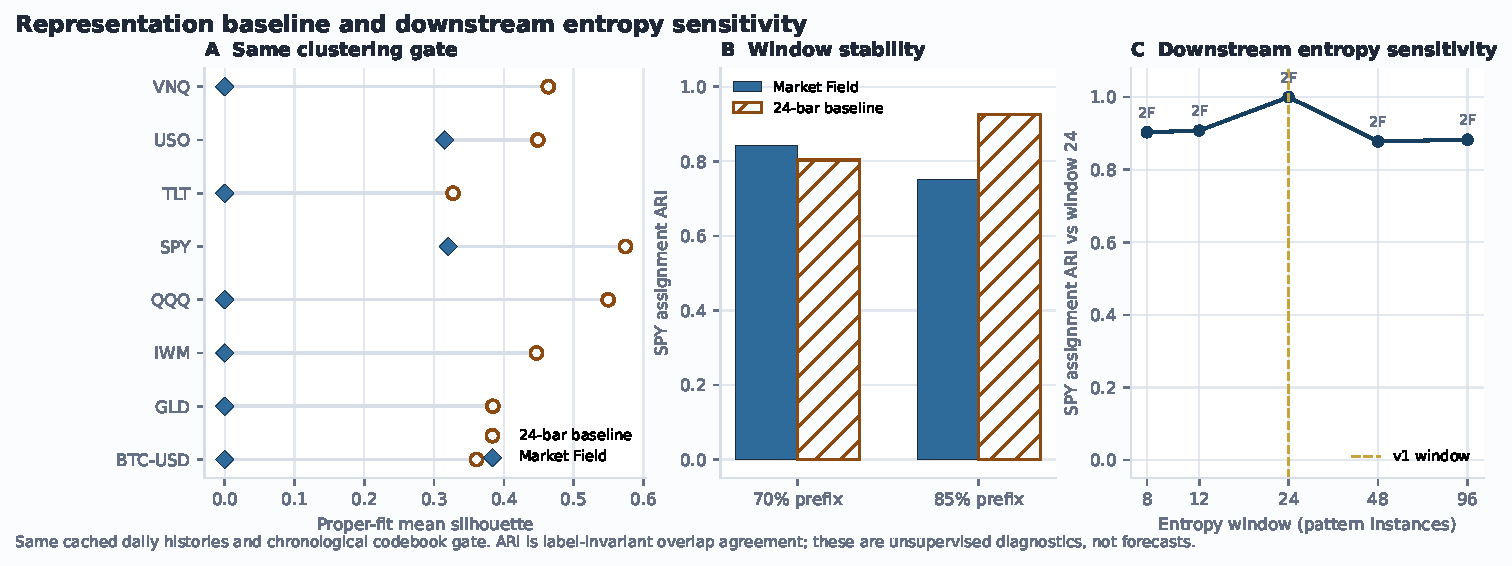
\includegraphics[width=\linewidth]{representation_sensitivity.pdf}
    \caption{The central negative and sensitivity evidence. The cheap baseline separates more readily under the same gate (A), prefix stability is mixed rather than dominated by \method{} (B), and SPY Form assignments are coarsely stable across entropy windows even while the underlying Information coordinate and distance tails move (C).}
    \label{fig:representation-sensitivity}
\end{figure}

The matched baseline accepts multi-Form codebooks for 8/8 assets with median proper-fit silhouette 0.448. \method{} accepts them only for SPY and USO, with median silhouette 0.000 because six one-Form fallbacks report zero. SPY prefix stability is mixed: \method{} assignment adjusted Rand index is 0.842/0.751 at the 70\%/85\% prefixes, versus 0.803/0.925 for the baseline. The complex vector therefore does not discover more separated or consistently more stable unsupervised states under this test. This result changes the role of the dictionary: it is a navigation and compression device over measured coordinates, not evidence of a superior latent representation.

Among 7,237 evaluation bars with state-conditional support, 395 enter the upper 5\% calibration-distance tail (5.46\% pooled), with asset rates from 1.51\% to 10.58\%; 33 USO rows are unsupported and excluded from the denominator. The heterogeneity matters more than the pooled proximity to 5\%.

\subsection{Expressiveness creates a sensitivity burden}

Changing only the permutation-entropy window leaves two long-history SPY Forms and assignment agreement of 0.878--0.908 against window 24, but the aggregate Information correlation falls to 0.492 at window 8 and 0.511 at window 96. Across the broader supplement, median alternative-window correlations are only 0.342--0.630 and the minimum is $-0.014$. SPY distance-tail rates move from 10.6\% to 16.7\%, and transitions move from 2.56 to 3.26 per 100 evaluation bars.

Horizon density is also a model choice. Relative to a dense step-1 grid over 8--64 bars, step 4 yields median correlation 0.940 but median IQR-normalized MAE 0.203 across 180 dataset--feature pairs; the 95th percentile is 0.428. Pressure is comparatively stable, while geometry and propagation move more. Retained history matters as well: 96 bars meets the input/support contract but produces median/p90 truncation error 0.035/0.931, versus approximately 0/0.003 at 365. Availability is therefore not convergence.

\section{Lessons from Building the Translation Layer}
\label{sec:lessons}

\paragraph{Auditability is necessary, not sufficient.}
Prefix consistency, deterministic replay, support masks, and receipts establish that the implementation can be inspected. They do not establish that a representation helps a decision. A retained-cache development runner reinforces this distinction: the raw 15D ridge has higher five-bar return MAE than the technical-24 comparator for 7/8 assets; SPY is worse by 0.00259 with a 95\% stationary-bootstrap interval $[0.00124,0.00395]$ and Holm-adjusted $p=0.016$. Every such row is marked development-only and decision-ineligible because the data had already informed construction.

\paragraph{Complexity is not the contribution.}
The cheap baseline forms cleaner clusters. Higher-order derivatives, entropy and Information, geometry and propagation, and the carrier ratios each add distinct sensitivity burdens under the reported tests. The durable contribution is that direction, change, organization, carriers, and comparison can be examined separately. A simpler family subset may ultimately be more useful and is now a predeclared ablation question rather than an aesthetic preference.

\paragraph{Missing support is part of the result.}
An unavailable coordinate, stale endpoint, beta-chain restart, or unmatched alignment key conveys information about what cannot be compared. Preserving gaps is more trustworthy than smoothing or forward-filling them into apparent continuity.

\paragraph{Comparison needs multiple bases.}
Native coordinate differences, own-history-relative differences, and relative price progress answer different questions. Keeping them separate prevents a large positive coordinate gap from being read as superior performance, leadership, or alpha.

\paragraph{The interface is part of the epistemic method.}
The research page now follows the same hierarchy as Figure~\ref{fig:research-contract}: conclusion, evidence, definition, audit. Progressive disclosure, one selected scope, synchronized dates, chronological trails, and explicit start/support/current markers reduce interpretive work without changing the numbers. This is a design rationale, not yet a usability result; a controlled comprehension study remains necessary.

\section{From an Auditable Instrument to a Prospective Study}
\label{sec:options}

The next goal is to test whether measured path context adds value to an already defined option-mispricing process. Optionality and path fit remain separate: cheapness, volatility edge, contract quality, execution quality, and recurrence determine the existing candidate score. A current field snapshot is computed only after eligibility and has zero direct weight; it cannot create eligibility, impose a veto, size, issue a verdict, or execute. Historical point-in-time field cohorts may enter a separately governed outcome-learning canary only when evidence gates and an operator gate pass, with all learning families together capped at 10\%. The event-level weight and marginal rank effect are receipted.

This implementation makes a prospective test possible today, but it does not supply its evidence retroactively. The repository freezes chronological origins, purging, outcomes, comparators, ablations, dependence-aware intervals, and multiplicity rules \citep{lopezdeprado2018advances,politisromano1994stationary}. The reserved study begins only after 2026-07-27 and requires at least 252 new observations before review. Any economic claim additionally needs point-in-time executable option quotes, spreads, slippage, commissions, assignments, normalized exposures, and predeclared primary endpoints. Historical impressions, complete option surfaces, and a genuinely untouched holdout cannot be reconstructed when they were never recorded.

Three priorities follow directly from the evidence:
\begin{enumerate}
    \item compare stable pressure/family subsets with the full 15D vector and cheap baselines under the frozen prospective protocol;
    \item test whether the conclusion--evidence--definition--audit hierarchy improves answer accuracy, time, and calibration for human readers; and
    \item extend beyond Pair v1 to point-in-time peer and sector baskets, cross-sectional ranks, and cross-timeframe panels only after constituent, session/currency, and per-cell support contracts are fixed.
\end{enumerate}
A feature is ready for promotion only if its decision-time input is reconstructible, its authority and failure modes are bounded end to end, and its evidence was not used to invent or tune it.

\section{Limitations}

The formulas contain hand-set constants, and the zero-field anchors are nonintuitive: coherence lies in $(7/27,1]$, Structure equals 0.42, and legacy display organization equals 0.68. High-order bounded differences amplify noise; row-adjacent smoothing changes with horizon density; the entropy estimator is short-window and parameter-sensitive; and 96 bars does not approximate full-history EWM state uniformly. Forms cluster reduced vectors rather than the complete field and remain request-window-relative.

Yahoo Finance histories are adjusted, revisable provider data rather than exchange truth. The live provider may expose a forming bar; audited option snapshots use completed prefixes. Volume coverage is not uniform, and exchange-session completion is not independently certified for every asset/timeframe. Pair comparisons inherit provider aliases, session, timezone, currency, adjustment, and selected-comparator limitations. Exact alignment keys and support make these issues visible but do not resolve them.

The evaluation establishes representation mechanics on retained paths. It does not establish causal market structure, forecast skill, option profitability, or autonomous decision quality. The development results are already exposed to model construction, option outcomes overlap, and historical ledgers lack the complete quote, exposure, cost, exercise, capacity, and impression record required for economic inference.

\section{Conclusion}

This work began with a practical problem: how to say what a market path is doing without collapsing it into one opaque score or presenting an unreadable wall of indicators. \method{} now provides a coherent answer at the measurement level. A conclusion can be traced through its horizon field, 15 defined coordinates, support, own-history context, chosen-reference comparison, and versioned self-checking receipt. Tested computations are prefix-consistent and deterministic, and controlled paths produce the intended distinctions.

The negative evidence is what makes that conclusion useful rather than promotional. More coordinates did not produce cleaner learned states than a cheap baseline, and entropy, resolution, and retained history materially affect the elaborate layers. The mathematics therefore earns no authority by being complex. Its present value is an auditable lens for inspection and a disciplined way to collect the next evidence. The next paper-worthy result is not another layer of terminology; it is a prospective answer to whether a simpler subset, relative comparison, or bounded path-context lean improves option decisions after costs---and whether human readers can reach better-calibrated conclusions with the translation hierarchy.

\section*{Reproducibility Statement}

Source, derived evidence, hashes, executed notebooks, environments, receipts, and bibliography audit are included. Formula v1 and semantic 1.3 identify the recipe, normalized input, support, and combined analysis, but not provider truth. Restricted raw snapshots require an independently matching provider response. The README records the named/anonymous build, implementation lineage, rerun commands, and exact replay limits.

\section*{Ethics and Intended Use}

This is exploratory research, not investment advice or autonomous trading. A display can influence a person even when algorithmic authority is zero. Prospective promotion therefore requires out-of-sample evidence, bounded authority, explicit human approval, and cost/risk review.

\bibliography{references}
\bibliographystyle{iclr2026_conference}

\appendix

\section{Version and Evidence Boundary}
\label{app:versions}

\begin{table}[h]
\centering
\small
\setlength{\tabcolsep}{4pt}
\begin{tabular}{lll}
\toprule
Name & What changes & What does not change \\
\midrule
Formula v1 & Field and 15-coordinate vector & Fixed within this paper \\
Semantic 1.3 & Coverage, identities, authority receipts & Formula values and stored history \\
Preliminary v2 & Evaluation harness & Not a v2 field model \\
Pair v1 & Two independently computed fields & Neither component formula \\
\bottomrule
\end{tabular}
\caption{Version names used in the paper.}
\label{tab:versions}
\end{table}

\texttt{market\_field\_calculus\_v1} fixes the formulas below.
\texttt{semantic\_revision=1.3} adds finite-computation and
full-dependency-support coverage, computation identities, and direct/indirect
authority receipts while retaining older payloads. \texttt{maturity} is only a
compatibility alias, not convergence. Relative Field Pair v1 is a separate
two-instrument receipt over independently computed formula-v1 fields.
\texttt{market\_field\_preliminary\_v2} names the evaluation harness, not a v2
field model.

\section{Complete Field Calculus}
\label{app:calculus}

\subsection{Boundedness and prefix argument}
\label{app:prefix-proof}

For Equation~\ref{eq:efficiency}, the triangle inequality bounds endpoint displacement by total path length. The map $x/(1+|x|)$ is bounded, prefix-initialized EWMs and the stated nonnegative row blends are convex, and past-only rolling windows and recursions preserve prefix measurability by induction in $t$. Clipping preserves the asserted unsigned bounds, while the declared zero-denominator cases close degenerate paths. This elementary argument establishes a property of the formulas, not causal inference; the endpoint audits test selected implementation paths.

\subsection{Input contract and pressure construction}

Experiments compute on retained histories before selecting the reported window. The interactive service may request additional past bars, but a provider can return fewer; response caps, exact prefetch rules, and transport behavior are operational contracts documented in the repository. Horizons are bar counts within one selected timeframe, and the system does not fuse timeframes into a single model.

Let $\epsilon=10^{-9}$, let unqualified $\clip$ mean $\clip_{[0,1]}$, and define $\phi(x)=x/(1+|x|)$. The unsigned numerical clip first maps NaN to 0, $+\infty$ to 1, and $-\infty$ to 0. For consecutive finite observations, an EWM of span $q$ follows
\begin{equation}
\EWM_q(x)_1=x_1,\qquad
\EWM_q(x)_t=(1-\alpha_q)\EWM_q(x)_{t-1}+\alpha_qx_t,
\quad \alpha_q=\frac{2}{q+1}.
\label{eq:ewm}
\end{equation}
All EWMs use pandas \texttt{adjust=False}, \texttt{ignore\_na=False}, and \texttt{min\_periods=0}; the executed receipt pins the dependency version. Output is NaN until the first finite value, which initializes the EWM. A later missing value repeats the prior output but advances the absolute-position decay. If $g$ missing positions follow an observed EWM $y_s$ and $x_{s+g+1}$ is finite, the next output is
\begin{equation}
y_{s+g+1}=\frac{(1-\alpha_q)^{g+1}y_s+\alpha_qx_{s+g+1}}
{(1-\alpha_q)^{g+1}+\alpha_q}.
\end{equation}
Thus Equation~\ref{eq:ewm} is the $g=0$ case; missing positions are not treated as zeros or simply removed from the time axis.
The normalizer coerces timestamps and OHLC values, requires finite strictly positive OHLC with $H_t\ge\max(O_t,C_t,L_t)$ and $L_t\le\min(O_t,C_t,H_t)$, drops invalid price rows, keeps the last duplicate timestamp, sorts rows, and reports every rejection category. Boundary comparisons accept only a tight \texttt{isclose} tolerance (relative and absolute tolerance $10^{-12}$) to avoid rejecting floating-point boundary noise. Invalid or missing volume does not discard a valid price bar; it becomes unavailable for volume-dependent carriers and its coverage is reported. At least 60 valid price rows must remain for the public field. This visible input-quality contract is part of current semantic revision 1.3.

True range follows Wilder \citep{wilder1978new}:
\begin{equation}
TR_t=\begin{cases}
H_t-L_t,&t=1,\\
\max(H_t-L_t,\ |H_t-C_{t-1}|,\ |L_t-C_{t-1}|),&t>1.
\end{cases}
\end{equation}
The true-range mean uses the available trailing $\min(h_j,t)$ observations. In Equation~\ref{eq:direction}, $z_{j,t}=0$ when that mean is zero. In Equation~\ref{eq:efficiency}, $e_{j,t}=0$ when the path sum is zero or $M_{t-h_j}$ is unavailable. Otherwise the triangle inequality makes clipping mathematically redundant. Let
$s_{j,t}=\EWM_5(d_{j,t}e_{j,t})$. The first adjacent-row blend is
\begin{equation}
q_{j,t}=0.68s_{j,t}+0.32N_j(s)_t,
\end{equation}
where $N_1(s)=s_2$, $N_J(s)=s_{J-1}$, and
$N_j(s)=(s_{j-1}+s_{j+1})/2$ in the interior (with $N_1(s)=s_1$ when $J=1$). After $x_{j,t}=\EWM_3(q_j)_t$, the second blend is
\begin{equation}
\pressure_{j,t}=0.58x_{j,t}
+0.42\frac{x_{j-1,t}+2x_{j,t}+x_{j+1,t}}{4},\qquad 1<j<J.
\end{equation}
At an edge, the bracketed neighborhood becomes $(2x_{\mathrm{edge}}+x_{\mathrm{neighbor}})/3$; for $J=1$, $\pressure=x$. These convex operations preserve the pressure bound. Equal row adjacency, rather than distance in $\log h$, is the declared v1 smoothing model.

\subsection{Base field channels}

Write $u_j=\log h_j$ and let $\mathcal G_u$ denote the same nonuniform-grid derivative used by \texttt{numpy.gradient(..., edge\_order=1)}. If $J=1$, the implementation sets both log-horizon derivative channels and the scaling exponent to zero. For $J\ge2$, endpoints use one-sided slopes. For an interior row, with $a=u_j-u_{j-1}$ and $b=u_{j+1}-u_j$,
\begin{equation}
(\mathcal G_uX)_j=
-\frac{bX_{j-1}}{a(a+b)}+\frac{(b-a)X_j}{ab}
+\frac{aX_{j+1}}{b(a+b)}.
\label{eq:scale-stencil}
\end{equation}
Let $R_1=\mathcal G_u\pressure$, $R_2=\mathcal G_uR_1$,
$G=1.35|R_1|/(1+1.35|R_1|)$,
$L=1.35|R_2|/(1+1.35|R_2|)$, and
$T=\clip(2.70|\Delta_t\pressure|)$, where the first temporal difference is zero. Then
\begin{align}
S&=\clip(1.8|\pressure|), &
Q&=\clip(1.4|v|),\\
B&=\clip(0.42G+0.33T+0.25L),&
Coh&=\clip(1-G/1.35),\\
E^{(0)}&=\clip(0.60(1-Coh)+0.40Q),&
E&=\EWM_4(E^{(0)}),\\
O&=\clip(0.48Coh+0.32S+0.20(1-E)).
\end{align}
Here $S,Q,B,Coh,E,O$ are state strength, velocity strength, boundary energy, coherence analogue, disorder analogue, and the legacy display channel serialized as \texttt{confidence}. Because $G\in[0,1)$, clipping is inactive in $Coh=1-G/1.35$ and $Coh\in(7/27,1]$. Consequently the $0.42Coh$ term in Structure contributes strictly more than $49/450\approx0.109$; Structure cannot reach zero under v1. The state-vector stratum called Structure is different from $O$. Under the zero field, $(S,Q,G,L,T,E)=(0,0,0,0,0,0)$, $Coh=1$, and $O=0.68$; this means agreement at zero and low disorder, not active organization. Further display channels are
\begin{align}
\mathrm{Expansion}&=\clip(1.8\,\operatorname{sign}(\pressure)v),\\
\mathrm{Contraction}&=\clip(-1.8\,\operatorname{sign}(\pressure)v),\\
\mathrm{Reflectivity}&=
\frac{\log(1+4\clip(0.50S+0.22Q+0.28B))}{\log 5},\\
\mathrm{Convection}&=\clip\big(B(0.45+0.55Q)\big).
\end{align}
These names are operational. Coherence is not spectral coherence; disorder is not generally information entropy; reflectivity is not optical reflectivity; and convection does not assert fluid dynamics.

\subsection{Research strata and carriers}

For any row field $Y$, define signed normalization and causal difference operators
\begin{equation}
\mathcal N_q(Y)_{j,t}=\phi\!\left(\frac{Y_{j,t}}{\EWM_q(|Y_j|)_t}\right),
\qquad
\mathcal D_q(Y)_{j,t}=\mathcal N_q(Y_{j,t}-Y_{j,t-1}),
\end{equation}
with first difference and result zero when the denominator is at most $\epsilon$. Thus $v=\mathcal D_{13}(\pressure)$, $a=\mathcal D_{13}(v)$, $j=\mathcal D_{13}(a)$, and $s_4=\mathcal D_{13}(j)$. The research scale channels are
\begin{equation}
g=\mathcal N_{13}(\mathcal G_u\pressure),\qquad
c=\mathcal N_{13}(\mathcal G_u\mathcal G_u\pressure),\qquad
m=\mathcal D_{13}(g),
\end{equation}
where every EWM normalizes along time, row by row. Thus $m$ is a bounded temporal difference of the bounded scale gradient, not a raw mixed partial.

Order-3 permutation entropy is evaluated separately on each pressure row. At time $t$, a stable sort maps $(\pressure_{j,t-2},\pressure_{j,t-1},\pressure_{j,t})$ to one of $3!=6$ possible ordinal patterns, with earlier positions winning ties. The plug-in distribution uses the most recent at most 24 observed pattern \emph{instances}:
\begin{equation}
H^{\mathrm{perm}}_{j,t}=-\frac{\sum_{\pi\in S_3}p_{\pi,j,t}\log p_{\pi,j,t}}{\log 6},
\end{equation}
with $0\log0=0$. Before two pattern instances exist, the value is zero. This short-window plug-in estimator is descriptive and can be downward biased; the material window sensitivity is reported in the main discussion. With bounded scale gradient $g$ and velocity $v$,
\begin{align}
c_{v,j,t}&=\tanh\left(-\frac{v_{j,t}g_{j,t}}{g_{j,t}^2+0.08}\right),\\
Pr_{j,t}&=\clip\left(1.8\sqrt{|v_{j,t}||g_{j,t}|}(0.45+0.55Coh_{j,t})\right).
\end{align}
The constant 0.08 is an engineered regularizer. For an idealized translating front $P(u,t)=F(t-\beta u)$, $P_t=F'$ and $P_u=-\beta F'$, so $-P_tP_u=\beta(F')^2$. This supports the sign convention---positive indicates motion toward larger horizons---but amplitude deformation can produce the same analogue.

The row-level strata are
\begin{align}
\mathrm{Structure}_{j,t}&=\clip(0.58S_{j,t}+0.42Coh_{j,t}),\\
\mathrm{Kinematics}_{j,t}&=\clip(0.18|v|+0.24|a|+0.27|j|+0.31|s_4|)_{j,t},\\
\mathrm{Geometry}_{j,t}&=\clip(0.32|g|+0.28|c|+0.20|m|+0.20B)_{j,t},\\
\mathrm{Information}_{j,t}&=\clip(0.72H^{\mathrm{perm}}_{j,t}+0.28E_{j,t}).
\end{align}
Define horizon-weighted and arithmetic reductions
\begin{equation}
\mathcal A_h(Y)_t=\frac{\sum_{j=1}^Jh_jY_{j,t}}{\sum_{j=1}^Jh_j},
\qquad
\mathcal A_0(Y)_t=\frac1J\sum_{j=1}^JY_{j,t}.
\label{eq:reductions}
\end{equation}
The five derivative coordinates use $\mathcal A_h$. Structure, Kinematics, Geometry, Information, and Propagation use $\mathcal A_0$, with
\begin{equation}
\mathrm{Propagation}_t=\mathcal A_0(Pr)_t,\qquad
\mathrm{CascadeBias}_t=
\begin{cases}
\dfrac{\sum_jPr_{j,t}c_{v,j,t}}{\sum_jPr_{j,t}},&\sum_jPr_{j,t}>\epsilon,\\
0,&\text{otherwise}.
\end{cases}
\end{equation}

Let $C_t^+=\max(C_t,\epsilon)$ and $r_t=\Delta\log C_t^+$ with $r_1=0$. Realized variation is
$RV_{j,t}=\sqrt{\sum_{i=t-h_j+1}^t r_i^2}$ over available observations, without annualization. The local scaling exponent is
\begin{equation}
\gamma_{j,t}=\clip_{[-2,2]}\left[\mathcal G_u\log(RV+\epsilon)\right]_{j,t},
\qquad \mathrm{ScalingExponent}_t=\clip_{[-2,2]}\mathcal A_0(\gamma)_t.
\end{equation}
It is not a Hurst exponent or multifractal spectrum. For equal per-bar squared variation, $RV_h\propto h^{1/2}$ and $\gamma\approx0.5$ is the natural reference. A value near 0 means accumulated variation changes little across the local scale neighborhood (for example, one common shock dominates), while 1 means approximately linear growth in $RV_h$. Because nested-window $RV_{j,t}$ is nondecreasing in $h_j$, $f_j=\log(RV_{j,t}+\epsilon)$ is nondecreasing. Endpoint one-sided secants are therefore nonnegative, and the interior stencil in Equation~\ref{eq:scale-stencil} equals
\begin{equation}
\frac{b}{a+b}\frac{f_j-f_{j-1}}{a}+\frac{a}{a+b}\frac{f_{j+1}-f_j}{b}\ge0.
\end{equation}
Thus $\gamma\ge0$ in exact arithmetic. The symmetric lower clip is only a defensive implementation guard: a materially negative preclip or emitted value is a numerical, unsorted-grid, inconsistent-window, or implementation-quality failure to investigate, not an interpretable state or evidence of anti-persistence. The service retains such a value only in its invalid diagnostic channel, withholds it from option translation, and suppresses the request's Form dictionary and retrospective relationship atlas so the impossible coordinate cannot influence a learned output.

Let $\widetilde V_t=V_t$ when volume is finite and nonnegative, and let it be unavailable otherwise. Define the pointwise impact observation
\begin{equation}
Z_t=\begin{cases}|r_t|/(C_t^+\widetilde V_t),&\widetilde V_t>0,\\
\mathrm{NaN},&\text{otherwise},\end{cases}
\end{equation}
so missing, invalid, and zero volume make that impact observation unavailable rather than zero. The row inputs
\begin{equation}
U_{j,t}=\operatorname{mean}_{i=t-h_j+1}^{t,\,\widetilde V_i\ \mathrm{available}}\widetilde V_i,
\qquad
I_{j,t}=\operatorname{mean}_{i=t-h_j+1}^{t,\,Z_i\ \mathrm{available}}Z_i
\end{equation}
use available observations only (pandas rolling means with \texttt{min\_periods=1}); either mean is unavailable when its window has no admissible observation. Here $I$ is Amihud-like \citep{amihud2002illiquidity}. For $X\in\{RV,U,I\}$ and $b=\max(34,2h_J)$, the bounded carrier field and separately displayed direct ratio are
\begin{align}
L_b(X)_{j,t}&=\clip\left[0.5+0.5\tanh\left(2\log\frac{X_{j,t}+\epsilon}{\EWM_b(X_j)_t+\epsilon}\right)\right],\\
R_b(X)_{j,t}&=\clip_{[0,10]}\frac{X_{j,t}+\epsilon}{\EWM_b(X_j)_t+\epsilon}.
\end{align}
The three state-vector carriers are $\mathcal A_0(L_b(RV))$, $\mathcal A_0(L_b(U))$, and $\mathcal A_0(L_b(I))$. The pandas EWM baseline is evaluated on the masked series and includes the current available observation. A direct ratio is unavailable wherever its current rolling input is unavailable; participation and impact ratios also require at least one positive-volume observation in the input. Missing internal carrier cells are filled with 0.5 only after this calculation to keep the optional retrospective clustering path finite: 0.5 is a neutral computational placeholder, not an observation, and must not be reported as a measured $1.0\times$ ratio. Impact cannot be observed from a zero-volume bar.

\section{Fixed Constants and Rationale}
\label{app:constants}

Table~\ref{tab:constants} inventories the principal hand-set constants. They were inherited from the deployed v1 design and fixed before the baseline and entropy analyses in this revision; that chronology prevents tuning to the new results but is not preregistration or evidence of optimality.

\begin{table}[h]
\centering
\footnotesize
\setlength{\tabcolsep}{3pt}
\begin{tabular}{p{0.24\linewidth}p{0.27\linewidth}p{0.42\linewidth}}
\toprule
Component & Constants & Design rationale / status \\
\midrule
Pressure time smoothing & EWM spans 5, 3 & Short causal denoising stages inherited from v1. \\
Pressure row blends & 0.68/0.32; 0.58/0.42 & Preserve own-row dominance while sharing adjacent scale context. \\
Base channel gains & 1.35, 1.4, 1.8, 2.70 & Map bounded visual analogues into useful display ranges; uncalibrated. \\
Motion normalization & EWM span 13 & Common causal scale for successive bounded differences. \\
Structure & 0.58 activity, 0.42 agreement & Hand-set composite; creates the disclosed nonzero floor. \\
Kinematics & 0.18/0.24/0.27/0.31 & Increasing weight on higher-order motion; not estimated. \\
Geometry & 0.32/0.28/0.20/0.20 & Balances gradient, curvature, mixed change, and boundary energy. \\
Information & 0.72 entropy, 0.28 disorder & Makes ordinal entropy load-bearing; sensitivity is explicitly tested. \\
Propagation & 0.08 regularizer; 1.8 gain; 0.45/0.55 agreement blend & Stabilizes the level-set analogue and emphasizes agreement. \\
Carriers & $b=\max(34,2h_J)$; ratio cap 10 & Longer causal reference than the largest configured horizon. \\
Metric families & 1/3 each & Equal total weight for derivatives, transforms, and carriers. \\
Dictionary gate & $k\le5$; max(20, 5\%) support; silhouette 0.25 & Conservative deterministic acceptance rule. \\
Signature & 0.35 bins & Coarse request-local identity; no semantic meaning. \\
Option hypotheses & 20-bar minimum; quantiles 35--75\% & Exploratory prior-row thresholds, not fitted classifiers. \\
Scanner base & 0.30/0.28/0.27/0.15; recurrence 0.12 & Pre-existing option heuristic; the current Market Field snapshot's direct base-score weight remains zero. \\
\bottomrule
\end{tabular}
\caption{Principal fixed constants. No listed value is inferred from the baseline or entropy-sensitivity outcomes.}
\label{tab:constants}
\end{table}

\section{Dictionary Chronology and Semantics}
\label{app:dictionary}

Using Equation~\ref{eq:reductions}, the exact state vector is
\begin{align}
\mathbf x_t=(&\mathcal A_h(\pressure),\mathcal A_h(v),\mathcal A_h(a),\nonumber\\
&\mathcal A_h(j),\mathcal A_h(s_4),
\mathcal A_0(\mathrm{Structure}),\mathcal A_0(\mathrm{Kinematics}),\nonumber\\
&\mathcal A_0(\mathrm{Geometry}),\mathcal A_0(\mathrm{Information}),
\mathrm{Propagation},\mathrm{CascadeBias},\nonumber\\
&\mathrm{ScalingExponent},\mathcal A_0(L_b(RV)),
\mathcal A_0(L_b(U)),\mathcal A_0(L_b(I)))\in\R^{15}.
\label{eq:state-vector}
\end{align}
The first five, next seven, and final three coordinates form derivative, field-transform, and OHLCV-carrier families.

For $N$ available rows, v1 uses zero-based split indexes
\begin{align}
t_E&=\max(5,\min(\lfloor0.60N\rfloor,N-6)),\\
t_F&=\min(w,\max(0,t_E-40)),\qquad w=\max(34,2h_J),\\
n_{cal}&=\min\{\max(20,\lfloor(t_E-t_F)/3\rfloor),\max(0,t_E-t_F-20)\},\\
t_C&=t_E-n_{cal}.
\end{align}
Proper fit is $[t_F,t_C)$, held-out distance calibration is $[t_C,t_E)$, and evaluation is $[t_E,N)$. Thus the fit and calibration segments retain at least 20 rows when the input guards permit. Scaling, codebook selection, centroids, and transition grammar use proper fit only; state-conditional distance references use calibration; evaluation supplies displayed sequences and descriptive forward annotations.

For feature $\ell$, proper-fit center is the median and initial scale is the interquartile range computed by NumPy quantiles with \texttt{method=linear}. If scale is at most $\epsilon$, fallback order is $1.4826$ times median absolute deviation, population standard deviation, and finally 1, each selected only when greater than $\epsilon$. Let $z_{t\ell}=(x_{t\ell}-m_\ell)/s_\ell$. Squared metric distance is
\begin{equation}
d(\mathbf x_t,\boldsymbol\mu)^2=
\frac1{15}\sum_{\ell\in\mathcal D}(z_{t\ell}-\mu_\ell)^2+
\frac1{21}\sum_{\ell\in\mathcal S}(z_{t\ell}-\mu_\ell)^2+
\frac1{9}\sum_{\ell\in\mathcal C}(z_{t\ell}-\mu_\ell)^2,
\label{eq:metric}
\end{equation}
where family sizes are 5, 7, and 3. Equivalently, coordinates are multiplied by the square root of their displayed weight before Euclidean $k$-means and silhouette computation.

For each candidate $k=2,\ldots,\min(5,\lfloor n_{fit}/n_{min}\rfloor)$, where $n_{min}=\max(20,\lceil0.05n_{fit}\rceil)$, the first seed is the fit point closest to the metric-space origin. Each later seed is the point farthest from its nearest existing seed; first row wins an exact tie. Lloyd updates run for at most 40 iterations, nearest-centroid ties choose the lowest index, and an empty cluster retains its previous centroid. Convergence requires unchanged assignments and centroids within absolute tolerance $10^{-12}$ and zero relative tolerance. The signature coordinate is $q_\ell=\texttt{np.rint}(\mu_\ell/0.35)$ cast to little-endian 32-bit integer; \texttt{rint} rounds to nearest integer with exact half ties to even. A candidate is discarded if any cluster lacks $n_{min}$ rows, any centroid separation is at most $10^{-6}$, two centroids share the same signature vector, or mean metric-space silhouette is below 0.25. The accepted candidate maximizes silhouette, with smaller $k$ winning a tie; if none passes, $k=1$. Final centroids are ordered lexicographically after rounding metric coordinates to 10 decimals. These choices are deterministic engineering rules, not evidence that the resulting Forms are natural latent states.

The reported legacy match transform uses the median of \emph{pooled} calibration nearest-centroid distances (falling back to fit distances only if calibration is empty):
\begin{equation}
\mathrm{match}_t=\exp\left(-d_t/\max(\med(d^{\mathrm{cal}}),\epsilon)\right).
\end{equation}
It is a monotone resonance transform, not a probability; the state-conditional empirical tail rank in Equation~\ref{eq:tail} is the more transparent distance context. Evaluation outcomes use overlapping windows and are not independent. Form names summarize calibration-relative measurement profiles; they are not universal economic regimes or concepts learned independently of the feature design.

\begin{table}[h]
    \centering
    \small
    \begin{tabular}{lrrrrr}
\toprule
Asset & Bars & Forms & Silhouette & Tail $n$ & Outside (\%) \\
\midrule
SPY & 2,148 & 2 & 0.320 & 860 & 10.6 \\
QQQ & 2,148 & 1 & 0.000 & 860 & 4.4 \\
IWM & 2,148 & 1 & 0.000 & 860 & 6.6 \\
TLT & 2,148 & 1 & 0.000 & 860 & 3.3 \\
GLD & 2,148 & 1 & 0.000 & 860 & 6.6 \\
USO & 2,148 & 3 & 0.315 & 827 & 6.8 \\
VNQ & 2,148 & 1 & 0.000 & 860 & 1.5 \\
BTC-USD & 3,124 & 1 & 0.000 & 1,250 & 4.4 \\
\midrule
Pooled & 18,160 & -- & -- & 7,237 & 5.5 \\
\bottomrule
\end{tabular}

    \caption{Daily-series dictionary diagnostics. Silhouette is zero when the support gate returns one Form. Tail $n$ counts evaluation bars with at least 20 state-conditional calibration references. The table's ``Outside'' column preserves the v1 legacy label and means upper 5\% calibration-distance tail.}
    \label{tab:assets}
\end{table}

\begin{figure}[h]
    \centering
    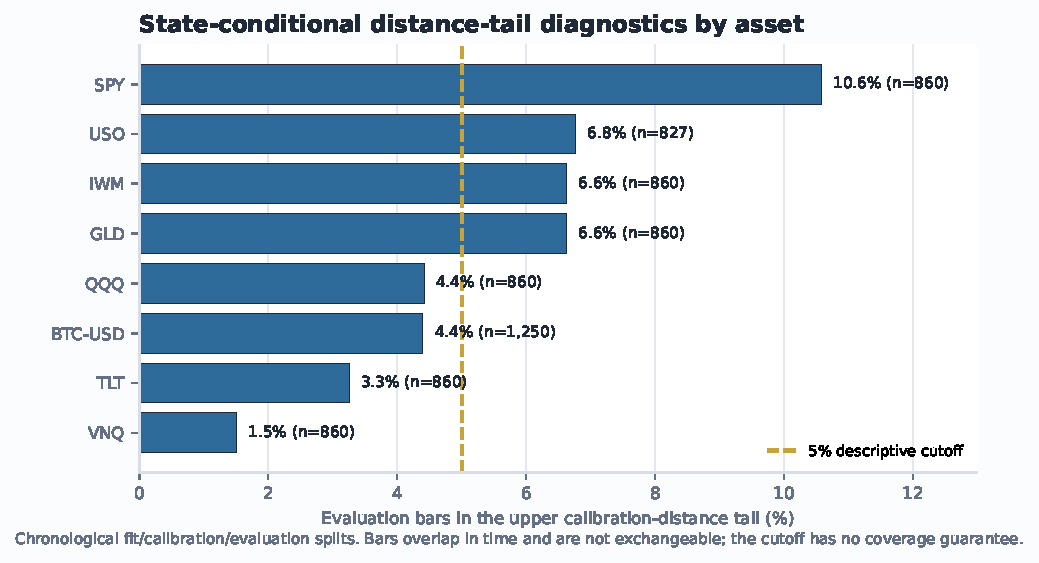
\includegraphics[width=0.88\linewidth]{calibration_rates.pdf}
    \caption{Asset heterogeneity in the empirical distance-tail diagnostic. The dashed line is a descriptive cutoff, not a promised coverage level.}
    \label{fig:tailrates}
\end{figure}

\section{Completed-Bar Option Contract}
\label{app:option}

The option snapshot retains at most 365 daily bars, requires at least 96, and treats a session as complete after 16:15 America/New\_York. It uses horizons $\{12,14,\ldots,48\}$ and excludes retrospective dictionary sections. The 96-bar threshold is the disclosed $2h_{\max}$ initialization target adopted after the truncation audit; snapshots with 60--95 bars are unavailable and report how many bars are still needed. Available snapshots also record alignment basis, input quality, authority, and a 15-row coordinate-coverage block. Each row separates a finite computed value from the per-time full-dependency-support mask and reports required inputs, the declared support lower bound, retained-prefix depth, current availability, and whether a finite internal neutral placeholder stands in for an unavailable carrier. Unavailable option responses carry canonical bars-needed metadata but no fabricated 15-row analysis block. \texttt{maturity} remains only a legacy serialized alias. These masks do not make the infinite-memory EWM identical to a full-history calculation. Support and resistance are strictly shifted:
\begin{equation}
\mathrm{Support}_t=\min_{i=t-20}^{t-1}L_i,\qquad
\mathrm{Resistance}_t=\max_{i=t-20}^{t-1}H_i.
\end{equation}
ATR is a trailing 14-bar simple mean of true range. Range position, close-to-SMA20, five-bar return, and ATR distance to the boundaries provide price-action context.

All hypothesis thresholds are computed from rows strictly before the current row and require at least 20 finite observations. Quantiles use NumPy's default linear interpolation:
\begin{itemize}
    \item \textbf{Organized expansion:} structure $\ge q_{70}$, propagation $\ge q_{60}$, information $\le q_{50}$, and $|p|\ge q_{60}$.
    \item \textbf{Longward cascade:} propagation $\ge q_{72}$, cascade bias $\ge\max(0.08,q_{62})$, and $|p|\ge q_{55}$.
    \item \textbf{Geometry/disorder shock:} geometry $\ge q_{75}$ and information $\ge q_{60}$.
    \item \textbf{Kinematic exhaustion:} kinematics $\ge q_{75}$, $|p|\ge q_{65}$, and pressure-aligned velocity $\widetilde v=\operatorname{sign}(p)v\le q_{35}$.
\end{itemize}
These are deterministic exploratory definitions, not trained classifiers. The legacy fallback assumes a long directional single-leg interpretation; semantic v1.3 instead prefers signed delta or opening action plus option type, and abstains for unsupported exposure rather than applying that fallback to a known short or multi-leg structure.

Each scanner component is an existing heuristic on $[0,100]$. Its base score remains
\begin{equation}
B=0.30\,\mathrm{cheapness}+0.28\,\mathrm{volEdge}
+0.27\,\mathrm{contractQuality}+0.15\,\mathrm{executionQuality}.
\end{equation}
For nonnegative integer recent-symbol, total-symbol, and recent-group counts $(s_r,s_T,g_r)$, the pre-existing recurrence component is
\begin{align}
R=\clip_{[0,100]}(&18\min(s_r,4)+4\min(\max(s_T-1,0),5)\nonumber\\
&+3\min(\max(g_r-s_r,0),6)),\qquad
\mathrm{rank}=\clip_{[0,100]}(B+0.12R).
\end{align}
\method{} has zero direct weight in both equations. Separately, let $\ell_f\in[0,100]$ be a reliability-weighted actual-close cohort score for available learning family $f$, including recurrence, replacement, Market Field, contract direction, and duration. A family is available only when the candidate cohort and at least one comparison cohort each contain at least eight closes. With normalized reliability weights $\alpha_f$ and mean reliability $\bar\rho$, the learning score and maximum proposed blend are
\begin{equation}
L=\sum_f\alpha_f\ell_f,\qquad
w=0.10\min(1,N/40)\min(1,q/0.10)\bar\rho,
\end{equation}
where $N$ is the count labeled as classified actual-close cycles and $q$ is their non-weak-process share. The applied score is $A=(1-w)\,\mathrm{rank}+wL$ only when $N\ge40$, $q\ge0.10$, at least one family is comparable, and the bounded canary is explicitly enabled by operator configuration; otherwise $A=\mathrm{rank}$ while the counterfactual remains observable. Thus 10\% is a hard total cap, not the Market Field family's weight. The policy cap cannot change automatically, although the event-level applied weight scales deterministically with the frozen evidence. The receipt decomposes each family's score contribution and leave-one-component-out rank effect.

In the manager, current field evidence may lower displayed advisory confidence or increase displayed urgency; because the decision window is rebuilt after that advisory change, urgency may also recompute \texttt{next\_review\_date}. It cannot change hard vetoes, verdicts, targets, sizing, or execution. The challenger remains unpromoted until at least 100 cycles, 25 additional new cycles, incremental out-of-sample value, and manual approval. Separate metamorphic tests compare supportive and contradictory contexts at the scanner/selection boundary and across stored-position, manager, and manual lifecycle-recording boundaries; within those tested boundaries, eligibility, selected contract, hard vetoes, target size, quantities, prices, P\&L, and execution authority remain invariant. This is not one continuous scanner-to-broker proof: the lifecycle test seeds the persisted event and contract, and the application does not own an automated broker execution path. Successfully finalized rank snapshots and authenticated browser impressions are append-only and idempotent from the independent rank/exposure-schema deployment boundary.

\section{Pairwise Relative Field Receipt}
\label{app:relative-pair}

Relative Field Pair v1 compares a target $A$ and benchmark $B$ only after each has been built independently under the same formula revision, timeframe, horizon grid, and settings. Let $X^A_{j,t}$ and $X^B_{j,t}$ be coordinate $j$ of the two 15-dimensional vectors and let $M^A_{j,t},M^B_{j,t}$ denote their source-observed, full-dependency-support masks. On an admissible aligned timestamp,
\begin{equation}
    \Delta^{\mathrm{native}}_{j,t}
    =X^A_{j,t}-X^B_{j,t},
    \qquad M^A_{j,t}=M^B_{j,t}=1 .
\end{equation}
Missing, provisional, invalid, or neutral-placeholder evidence is not coerced to zero. The sign means target minus benchmark in that coordinate's implemented 15-dimensional scale, not raw market units; it is not a utility ordering. In particular, the three carrier coordinates are bounded causal-baseline relative levels rather than raw realized variation, volume, or impact. Higher disorder, propagation, realized-variation state, participation, or liquidity stress is not inherently better.

Each component dictionary retains its own proper-fit location $m^q_j$ and robust scale $s^q_j$, $q\in\{A,B\}$. Pair context is
\begin{equation}
    \Delta^{\mathrm{context}}_{j,t}
    =\frac{X^A_{j,t}-m^A_j}{s^A_j}
     -\frac{X^B_{j,t}-m^B_j}{s^B_j}.
\end{equation}
It is emitted only on the intersection of the two evaluation segments, after both fixed proper-fit and held-out calibration partitions. Fit or calibration bars are not retrospectively displayed with those later reference statistics, and an unavailable scale remains unavailable. Thus the displayed context trace uses no future observation relative to its evaluation bar, but it remains request-window-relative: changing either retained history can change the two references. Request-local Form IDs and centroids are never matched across symbols.

Price progress is separate from field geometry. It uses the full-precision normalized close path carried beside each component analysis rather than the four-decimal display serialization. If $p^A_0,p^B_0$ are the first common aligned closes, the displayed relative index is
\begin{equation}
    RI_t=100\frac{p^A_t/p^A_0}{p^B_t/p^B_0}.
\end{equation}
Active progress is $RI_t-100$. For the separate beta-adjusted path, let $r^q_t=\log(p^q_t/p^q_{t-1})$. Once at least 20 prior aligned return pairs exist, $\widehat\beta_{t-1}$ is the centered covariance/variance slope---equivalent to the slope from an intercept-inclusive fit---over at most the 60 pairs strictly before $t$. The displayed increment is $r^A_t-\widehat\beta_{t-1}r^B_t$; it does not subtract the fitted intercept and is therefore not an OLS abnormal-return residual or alpha. The estimate is unavailable if the benchmark population return standard deviation is below $10^{-7}$, if the result is nonfinite, or if $|\widehat\beta_{t-1}|>25$. An invalid estimate is rejected rather than clipped or carried forward: the row's beta-adjusted return is unavailable and the cumulative chain resets, with any later valid estimate starting a new chain. The current beta/return summary uses the latest aligned row only and is unavailable whenever its beta is unavailable. The displayed cumulative beta-adjusted return is $100\{\exp[\sum_u(r^A_u-\widehat\beta_{u-1}r^B_u)]-1\}$ within each contiguous available chain. It is not used to transform field coordinates. Neither $RI_t$ nor a beta-adjusted return changes a Form or supplies a field ``winner.''

The alignment receipt declares its rule, per-leg dropped-observation counts at or after the displayed window start, and separately identified unmatched-tail counts. Those tails are subsets of the dropped counts; pre-window truncation is not counted as pair dropout. Daily and weekly rows align by serialized market-session date; the service does not independently certify exchange calendars or timezones. When intraday source timestamps retain timezone information, both sides normalize to UTC and require exact equality. Timezone-naive provider/cache rows instead require exact equality of their serialized naive timestamps and are not relabeled as UTC. Neither branch uses a nearest-neighbor join or forward fill, and matching timestamps do not certify common sessions: nonidentity pairs retain unknown session compatibility. Nonidentity DXY comparisons at 1h, 2h, and 4h are explicitly unavailable under the current provider anchors; DXY/DXY remains an algebraic identity control. The live endpoint uses provider/cache rows as returned and does not independently certify its latest bar as exchange-complete. The canonical \texttt{DXY} selector resolves to Yahoo's \texttt{DX-Y.NYB} index identifier and retains that alias in provenance; \texttt{UUP} is not substituted. Provider, adjustment, currency, timezone, and session differences remain comparison limitations.

The ordered comparison hash binds the target analysis hash, benchmark analysis hash, alignment contract, and normalization contract. Swapping $A$ and $B$ changes the receipt and reverses signed differences. The compact own-history-relative separation summary takes the same supported-coordinate intersection at $t$ and $t-5$, averages absolute context gaps within each of the three coordinate families, and then averages the family means. It is unavailable when any family lacks common support; a change no larger than $\max(0.05,0.05S_{t-5})$ is labeled \texttt{mixed} in the machine payload and translated as ``No clear net change.'' The payload also returns both stretch values, their change, tolerance, lookback, and contributing support. A deterministic descriptive summary adds no fitted score, and a separately hashed self-checking compact receipt binds exact shared keys, latest values, compatibility disclosures, and zero authority; it is unkeyed, is not digitally signed, and omits complete chart histories. The Overview names all-window and current support separately, states the exact relative-index base date, and labels the comparator's user-selected reference role with suitability unevaluated.

The reader-facing hierarchy is Overview, Field detail, and Audit receipt. Field detail mounts one of four scopes at a time, with all 15 coordinate histories available on demand; audit groups are collapsed until requested. Target, benchmark, and difference use solid/circle, dashed/diamond, and dotted/square encodings in addition to hue. Trail opacity is computed from source chronology rather than horizontal screen position, while bounded display simplification preserves supported endpoints and turns. Unsupported intervals remain broken or hatched, synchronized inspection uses shared dates, and \textsc{start}, \textsc{first supported}, \textsc{now}, and \textsc{latest supported} appear only when their distinct conditions hold. The default inspection scale may zoom the selected trail; an explicitly linkable shared scale preserves subject comparability. These presentation controls alter neither analytical values nor identities. The paths are visual projections, not detected cycles, attractors, lead--lag estimates, or connectedness.

Request-local backend timings and bounded browser events are operational instrumentation excluded from analytical identities; they are not chart-interaction measurements or a durable human-exposure ledger. Pair v1 has zero scanner, canary, veto, verdict, sizing, or execution authority. Basket fields, cross-sectional peer ranks, persistent cross-symbol Forms, cross-timeframe fusion, predictive value, and economic value remain future work. The present paper adds this auditable implementation boundary but no Pair-v1 efficacy result. A standalone reconstructibility supplement, \texttt{relative-field-addendum.tex}, specifies the exact alignment, precision, beta-adjustment, separation, receipt, and failure contracts.

\section{Cross-Market Shadow Atlas}

The research page can read cached energy, real estate, agriculture, metals, sector-divergence, and crypto measures. For each source, it screens Spearman association \citep{spearman1904association} between source pressure change and daily target log return at lags 0, 1, 5, and 20. The first 70\% selects the largest absolute association. Holdout inference uses 199 fixed-block permutations of ranked source values with block length five and Benjamini--Hochberg correction \citep{benjaminihochberg1995fdr}. This controls false discovery rate under its assumptions, not family-wise error rate. A relationship is called persistent only when calibration and holdout signs agree, holdout $|\rho|\ge0.15$, and $q\le0.10$.

This atlas is explicitly \texttt{shadow\_only} with no field influence. It is association screening, not evidence of a spillover mechanism. Sources have heterogeneous cache vintages and are daily even when the selected field is intraday. The option snapshot intentionally excludes them until stronger alignment, provenance, and prospective validation exist.

\section{Multi-Timeframe and Resolution Sensitivity}
\label{app:resolution}

The supplementary locally retained snapshot contains 9,235 completed bars across 15 datasets: SPY at 1m, 5m, 15m, 30m, 1h, 2h, 4h, 1D, and 1W, plus six additional daily markets. It excludes 15 latest rows under a conservative completion policy and finds zero duplicate timestamps, missing OHLCV cells, or invalid OHLC rows. All 46 prefix checks, including a direct mutation of the unseen SPY suffix, have zero error across 24,472 full-precision numeric values at tolerance $10^{-12}$; all 16 repeated canonical-hash checks match. The audit covers live matrices and aggregate derivatives, strata, carriers, and ratios while bypassing response rounding. Every evaluated channel is finite across all nine timeframes. These are availability and implementation-invariance results, not evidence that one parameterization transfers economically across sampling frequencies.

For grid sensitivity, step 1 over horizons 8--64 is the reference and steps 2, 4, and 8 are recomputed from the same completed prefixes. The audit discards $W=\min(128,\max(60,\lfloor N/3\rfloor))$ startup rows. For reference series $y$ and candidate $\widehat y$, it reports
\begin{equation}
\mathrm{NMAE}_{IQR}=\frac{\mean_t|y_t-\widehat y_t|}{Q_{0.75}(y)-Q_{0.25}(y)},
\end{equation}
where $Q_{0.25}$ and $Q_{0.75}$ use NumPy \texttt{method=linear} on pairwise-finite reference values; the statistic is unavailable when their difference is at most $10^{-9}$. Grid and entropy-window correlations are Pearson product-moment coefficients from \texttt{numpy.corrcoef} after pairwise deletion of nonfinite values. A correlation is unavailable with fewer than three pairs or when either population standard deviation is at most $10^{-12}$; aggregate medians and percentiles omit unavailable values and use linear interpolation. Across 15 datasets and 12 aggregate features, step 4 contains 180 pairs and produces median correlation 0.940 and median NMAE$_{IQR}$ 0.203; its 95th-percentile error is 0.428. All three coarser grids together contain 540 pairs. The worst step-4 pair is the SPY 15m scaling exponent (NMAE$_{IQR}$ 0.730, correlation 0.911). This does not define an optimal grid. It demonstrates that convergence must be measured per channel and that denser horizon resolution cannot be described as a purely visual enhancement.

Dictionary stability depends on sample length. On the 749-bar supplementary SPY daily window, the 70\% prefix selects one Form while the full window selects two, producing adjusted Rand index \citep{hubertarabie1985comparing} 0.000 on their overlap; the 85\% prefix and full window both select two and achieve 0.873. On the longer 2,150-bar primary SPY history, both prefixes retain two Forms but ARI is 0.842 at 70\% and 0.751 at 85\%. The matched single-horizon baseline yields 0.803 and 0.925. Shorter-window SPY and QQQ upper calibration-distance-tail rates are 36.7\% and 42.7\%, versus 10.6\% and 4.4\% in the longer primary sample. These differences are direct evidence that Form identity and empirical distance ranks are window- and distribution-dependent. Only two next-state entries meet the current reliability support across seven supplementary daily dictionaries.

A live operational probe artifact records HTTP 200 for all nine timeframe selectors and its run-specific endpoint timings, but conservatively flagged all latest provider bars as possibly forming. Consequently, paper results use locally retained completed prefixes. Live endpoint availability and timing are reported only as an operational check, not a stable performance distribution.

\section{Evaluation Details and Threats to Validity}

\paragraph{Synthetic construction.}
The deterministic reversal series contains 800 bars, a positive log drift before bar 400 and a negative drift afterward, with fixed OHLC ranges and volume. Threshold delay is the first post-reversal bar where $\pressure_{h,t}<-0.05$. The trend/chop contrast holds bar ranges and deterministic generation fixed while changing directional path organization. These tests are useful precisely because the expected behavior follows from construction; they do not estimate generalization.

\paragraph{Prefix audit.}
For each of eight daily series and four cut points, the primary script rebuilds both the prefix and full history. It compares 11 four-decimal serialized channels over 19 horizon rows at the matching final prefix timestamp. The supplementary full-precision audit expands live numeric coverage as described above. Zero difference means the tested paths did not use the later suffix; it does not prove causal inference, provider timestamp correctness, or absence of bugs outside those paths. Remaining regression scope includes minimum-input/initialization-coverage metadata, hypothesis flags, lexicon fields under a fixed split, and the complete final option snapshot.

\paragraph{Distance tails.}
The pooled rate in Table~\ref{tab:validation} is descriptive. Bars are serially dependent; calibration sizes vary by state; the same hyperparameters were developed while observing related markets; and distributions drift. Asset-level dispersion in Figure~\ref{fig:tailrates} is more informative than the pooled proximity to 5\%.

\paragraph{Operational benchmark.}
Timing uses one local Windows process with imports already loaded and cached in-memory histories. The supplementary distribution contains 63 warm runs across seven symbols; it excludes retrieval, persistence, fresh-process import time, concurrent load, network, and production queueing. It cannot be compared directly to production request latency or a service-level objective.

\paragraph{Data quality.}
Yahoo Finance adjusted OHLCV is convenient and reproducible only up to provider revisions. It is not the live IBKR path used by every application request. Corporate-action adjustments alter historical levels. The package therefore records canonical row hashes and never presents the sample as immutable exchange truth. Raw snapshots are retained locally but not redistributed; a fresh provider retrieval is a new sample even when its requested ticker and dates match.

\section{Research Progression and Design Rationale}

\begin{enumerate}
    \item \textbf{Horizon strips.} The starting point applied a common indicator across lookbacks, preserving SwamiCharts' visual scan across scale.
    \item \textbf{Continuous pressure.} Indicator votes were replaced with a signed, efficiency-weighted displacement so direction and organization remained continuous.
    \item \textbf{Causal derivatives.} Pressure change and successive bounded differences exposed strengthening, fading, and high-order instability without future bars.
    \item \textbf{Scale geometry and information.} Derivatives over log horizon, boundary energy, and ordinal entropy separated across-scale fragmentation from within-scale motion.
    \item \textbf{Field cloud and scopes.} A narrow horizon cloud became the overview; phase projections moved detailed relationships out of linear metric cards.
    \item \textbf{Translation layer.} A deterministic request-local codebook attached compact names to measured profiles while exposing support and range evidence.
    \item \textbf{Context atlas.} Prior-bar boundaries, option snapshots, and cached cross-market associations were added as visibly separate evidence layers.
    \item \textbf{Relative Field Pair.} Two independently computed same-recipe fields can be compared through shared-support coordinate differences, relative price context, and common-axis scopes without matching request-local Forms or granting the pair decision authority.
    \item \textbf{Prospective options instrumentation.} Immutable snapshots entered scanner and manager workflows with zero direct field weight, bounded indirect learning, and no execution authority, creating a path to future evaluation without silently changing eligibility.
\end{enumerate}

This progression is a design synthesis of established ideas, not a claim of new market physics. Its most important property is traceability: a phrase in the interface can be mapped back to a versioned vector, a completed data prefix, and explicit transformations.

\section{Economic-Evaluation Protocol and Remaining Evidence}
\label{app:future}

The repository now includes a machine-readable development protocol and deterministic prequential runner. It freezes chronological origins, fit/calibration/evaluation windows, purge/embargo, endpoints, methods, and a trial registry; reports unsupported rows separately; compares naive, EMA, technical, fixed two-window break, fit-only two-state diagonal-Gaussian HMM, raw-15D, dictionary, and family-ablation variants; uses a documented stationary bootstrap \citep{politisromano1994stationary}; and emits Benjamini--Hochberg and Holm adjustments rather than conflating exploratory FDR with confirmatory family-wise control. Its receipted dry run uses eight retained daily datasets (18,160 bars), 544 expanding purged origins, 11 model variants, and three future-only outcomes at 1, 5, and 20 bars. Exactly 53,361 of 53,856 unique cases are scored and 495 not-yet-observable targets remain explicitly pending; all split chronologies pass and no scored row is nonfinite or duplicated. Every HMM fit reached the protocol-specified cap of eight EM iterations without satisfying the source-fixed $10^{-6}$ relative stopping tolerance, so it is a cap-truncated fit-only comparator rather than a converged latent-state result. Five seeded IID, AR(1), alternating-return, volatility-shift, and missing-volume processes are construction checks only. The retained-cache run is development-only because those data have already informed construction.

A preregistered confirmatory study must still define a frozen universe, start date, option entry rule, holding horizon, and no-touch final holdout. At each origin, all scaling, thresholds, codebooks, and optionality baselines must be refit using only admissible history. The purge/embargo must cover the maximum holding horizon \citep{lopezdeprado2018advances}. Primary endpoints must be stated before inspection and include both statistical and economic measures. The frozen development runner provides a mechanism for this study; it does not make the retained cache untouched.

The current runner implements price/volume technical features, a single-horizon EMA system, a deterministic cap-truncated fit-only two-state HMM, and fixed causal location/scale/range/volume break scores. The last is a break-feature ridge, not a breakpoint estimator. A better-converged or sticky HMM, formal structural-break or Bayesian change-point model, wavelet/scattering, and sliding-window persistent-homology comparators \citep{pereaharer2015sliding,gideakatz2018tda} remain future because their fitting, transform, prior, scale-bank, and boundary choices must be frozen rather than selected after inspecting this development sample. IV-minus-realized-volatility and cross-market connectedness also remain future because the retained single-symbol OHLCV files lack point-in-time surfaces and aligned panel vintages. Existing ablations remove each field family and compare dictionary labels with the raw continuous vector.

Option outcomes require executable bid/ask observations, commissions, slippage, stale-quote controls, exercise conventions, and normalization by maturity, moneyness, delta, vega, exposure, and holding period. Dependence-aware bootstrap intervals and a predeclared multiplicity procedure must accompany repeated variants; the study must state whether it targets exploratory FDR or confirmatory family-wise error. A positive retrospective average is insufficient for promotion.

\section{Implementation Scope and Non-Claims}

The repository does not implement causal or connectedness estimators, persistent Forms, basket or cross-sectional fields, timeframe fusion, historical option surfaces, or validated execution. Pair v1 compares two same-recipe fields. Canvas2D smoothing does not estimate contours or attractors. Display work is engineering; state identity, causal fusion, option profitability, and execution require new evidence. \texttt{FUTURE\_WORK\_TRIAGE.md} records the fuller boundary.

Accordingly, the paper does not claim universal states, attractors, cycles, arbitrage, predictive return skill, profitable option selection, cross-market causation, or autonomous decision quality. The words \emph{causal} and \emph{prospective} refer respectively to non-anticipative prefix computation---not causal inference---and time-stamped future evaluation.

\section{LLM Usage Statement}

OpenAI Codex assisted repository and formula inspection, code, figures, literature organization, LaTeX drafting, and consistency review. The human author remains responsible for every claim, citation, artifact, and numerical result. This use must appear in the ICLR submission form; model output is neither evidence nor authorship.

\end{document}
